%\documentclass[notes]{beamer}
%\documentclass{beamer}
\documentclass[t,xcolor={dvipsnames,usenames}]{beamer}
%\documentclass[notes=only]{beamer}
%\setbeameroption{show only notes}

%\makeatletter
%\def\beamer@framenotesbegin{% at beginning of slide
%    \gdef\beamer@noteitems{}%
%      \gdef\beamer@notes{{}}% used to be totally empty.
%}
%\makeatother


\iffalse
\mode<presentation>
{  %\usetheme{Antibes}
   %\usetheme{JuanLesPins}
   \usetheme{Boadilla}
   %\usetheme{Montpellier}
   \setbeamercovered{transparent}
}
\setbeamertemplate{footline}
{
  \leavevmode%
  \hbox{%
        \begin{beamercolorbox}[wd=.4\paperwidth,ht=2.25ex,dp=1ex,center]
          {author in head/foot}%
          \usebeamerfont{author in head/foot}
          \insertshortauthor
        \end{beamercolorbox}%
        \begin{beamercolorbox}[wd=.6\paperwidth,ht=2.25ex,dp=1ex,center]
          {title in head/foot}%
          \usebeamerfont{title in head/foot}
          \insertshorttitle\hspace*{3em}
          \insertframenumber{} /
          \inserttotalframenumber\hspace*{1ex}
        \end{beamercolorbox}
  }%
  \vskip0pt%
}

\setbeamertemplate{navigation symbols}{}
\fi

%------------------------------------------------------------------------

% GK edits from shaden talk
\usetheme{default}

\setbeamersize{text margin left=.3in,text margin right=0.3in}
\setbeamertemplate{navigation symbols}{}

\setbeamercolor{title}{fg=black}
\setbeamercolor{section in toc}{fg=black}

\setbeamercolor{frametitle}{fg=black}
\setbeamerfont{frametitle}{series=\bfseries,size=\Large}
\setbeamertemplate{frametitle}
{ \vspace{4pt}
    \noindent\begin{minipage}[c][1.1em][t]{\textwidth}\insertframetitle\end{minipage}\par
      \hrule height 1pt\par
    }

    \setbeamercolor{block title}{fg=black}
    \setbeamercolor{itemize item}{fg=black}
    \setbeamercolor{itemize subitem}{fg=black}
    \setbeamercolor{enumerate item}{fg=black}
    \setbeamercolor{enumerate subitem}{fg=black}
    %\setbeamertemplate{itemize item}{{\small $\bullet$}}


    \setbeamercolor{footline}{fg=gray}
    \setbeamerfont{footline}{size=\Tiny}
    \setbeamertemplate{footline}
    {
      \flushright{\insertframenumber{} /
      \inserttotalframenumber\hspace*{2ex}}\par
      \vspace{1.5ex}\par
    }




%-----------------------------------------------------------------------

\usepackage{pgfpages}
\usepackage{bm} 
\usepackage{amsmath}
\usepackage{xspace}
\usepackage{graphicx}
\usepackage{threeparttable}
\usepackage{algorithm}
\usepackage{algpseudocode}
\usepackage{multirow}
\usepackage{url}

%\setbeamertemplate{note page}[plain]
%\setbeameroption{show notes on second screen=right}
%\setbeameroption{show notes on second screen=bottom}

%\graphicspath{{/home/grad02/mohit/exmoh/dev/bitbucket/thesisproposal/lfs/figures/}{/home/grad02/mohit/exmoh/dev/bitbucket/thesisproposal/matrixcompletion/figures/}{/home/grad02/mohit/exmoh/dev/bitbucket/thesisproposal/figures/}{/home/grad02/mohit/exmoh/dev/bitbucket/thesisproposal/bilinear/ope_slide/}{lfsnewfigures/}}


\graphicspath{{/Users/mohitsharma/dev/bitbucket/thesisproposal/lfs/figures/}{/Users/mohitsharma/dev/bitbucket/thesisproposal/matrixcompletion/figures/}{/Users/mohitsharma/dev/bitbucket/thesisproposal/figures/}{/Users/mohitsharma/dev/bitbucket/thesisproposal/bilinear/ope_slide/}{lfsnewfigures/}}

\DeclareGraphicsExtensions{.pdf,.png}
%\usepackage[backend=bibtex]{biblatex}
%\usepackage[style=authoryear]{biblatex}
\usepackage[
  backend=biber,
  style=alphabetic,
  citestyle=authoryear 
]{biblatex}
\bibliography{/home/grad02/mohit/exmoh/dev/bitbucket/thesisproposal/refs}
%\bibliography{/Users/mohitsharma//dev/bitbucket/thesisproposal/refs}
%\bibliographystyle{plain}
%\renewcommand*{\nameyeardelim}{\addcomma\addspace}

\newcommand*{\ML}{Movielens\xspace}
\newcommand*{\ARM}{ARM\xspace}
\newcommand*{\ES}{ESARM\xspace}
\newcommand*{\ESEXP}{Extremal subset average rating model\xspace}
\newcommand*{\VO}{VOARM\xspace}
\newcommand*{\VOEXP}{Variance offset average rating model\xspace}
%\newcommand*{\MXMN}{MXMNARM\xspace}
\newcommand*{\MLREALSETS}{ML-RealSets\xspace}
\newcommand*{\SYNSETSA}{SynSets\xspace}
\newcommand*{\SYNSETSB}{SynStdDev-1\xspace}
\newcommand*{\SYNSETSC}{SynStdDev-2\xspace}
\newcommand*{\SYNSETSD}{SynStdDev-3\xspace}
\newcommand*{\TOPN}{Top-$n$\xspace}
\newcommand*{\topf}{top $5\%$\xspace}
\newcommand*{\MLTM}{Movielens 20M\xspace}
\newcommand*{\MLOM}{Movielens 1M\xspace}
\newcommand*{\YMusic}{Yahoo Music\xspace}
\newcommand*{\YMovies}{Yahoo Movies\xspace}
\newcommand*{\BX}{Book-Crossing\xspace}
\newcommand*{\FLIX}{Flixster\xspace}
\newcommand*{\NF}{Netflix\xspace}
\newcommand*{\EM}{EachMovie\xspace}
\newcommand*{\JEST}{Jester\xspace}
\newcommand*{\MF}{Matrix Factorization\xspace}
\newcommand{\minimize}{\operatornamewithlimits{minimize}}

\newcommand\Fontvi{\fontsize{9}{9.2}\selectfont}

\title{Learning from sets of items in Recommender Systems}
\author{Mohit Sharma\\Advisor: Prof. George Karypis}
\institute{
  University of Minnesota\\
  \url{mohit@cs.umn.edu}
}
\date{\today}


%\AtBeginSection[]
%{
%  \begin{frame}[noframenumbering]{Table of Contents}
%    \tableofcontents[currentsection, sectionstyle=show/shaded]
%  \end{frame}
%}

\AtBeginSubsection[]
{
  \begin{frame}[noframenumbering]{Outline}
    \tableofcontents[currentsection, currentsubsection,
    sectionstyle=show/shaded, subsectionstyle=show/shaded]
  \end{frame}
}

%\AtBeginSubsubsection[]
%{
%  \begin{frame}[noframenumbering]{Table of Contents}
%    \Fontvi \tableofcontents[currentsection, currentsubsection,
%    sectionstyle=show/shaded, subsectionstyle=show/shaded]
%  \end{frame}
%}

\begin{document}
\begin{frame}
  \titlepage
\end{frame}

\begin{frame}[noframenumbering]{Outline}
   \tableofcontents
\end{frame}

\section{Overview}

\subsection{Recommender systems}
\begin{frame}{Recommender systems}
  \begin{itemize}
    \item Help consumers by providing suggestions that are expected to satisfy
      their tastes.
  \end{itemize}
  \begin{center}
  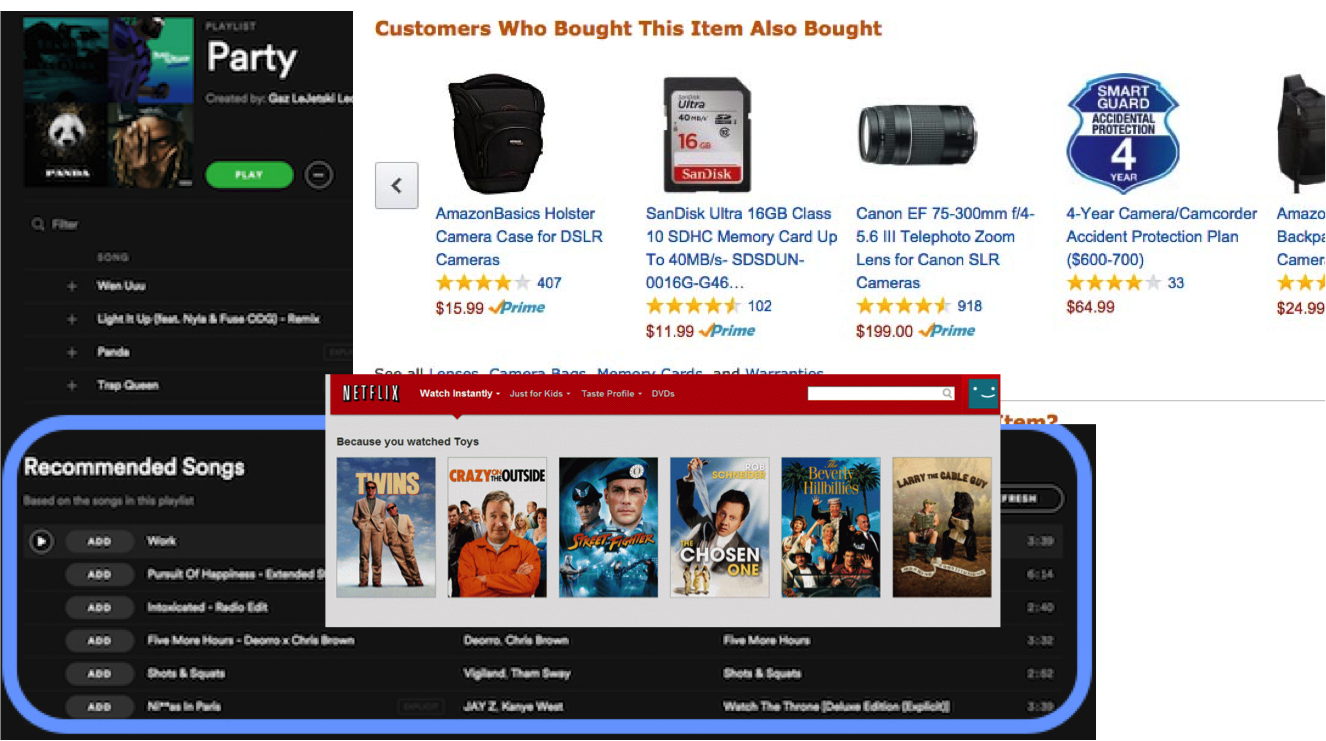
\includegraphics[scale=0.5]{recsys.png}
\end{center}
\end{frame}

\subsection{Factorized bilinear similarity}
\begin{frame}{Factorized bilinear similarity}
  \begin{itemize}
    \item Factorized bilinear similarity models for cold-start \TOPN item recommendations (SDM'15).
        \begin{equation*}
          \begin{split}
            sim(i,j) &= f_i ^T W f_j \\  
              &= f_i ^T ( D + V^T V) f_j\\
          \end{split}
        \end{equation*}
  \end{itemize}
  \begin{center}
    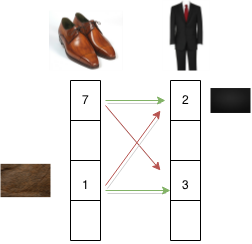
\includegraphics[scale=0.5]{fabric}
  \end{center}
\end{frame}


\begin{frame}{Factorized bilinear similarity}
  
  
  \begin{itemize}
    \item Preference of the user $u$ for a new item $i$ is given by:
      \begin{equation*} 
        \begin{split}
           \tilde{r}_{u,i} &= \sum_{j\in \mathcal{R}_u^+} sim(i,j) , \\
                           &= \sum_{j\in \mathcal{R}_u^+} f_i ^T D f_j + f_i ^T
          V^TV f_j
        \end{split}
      \end{equation*}   
    \item Bayesian personalized ranking (BPR) loss
      \begin{equation*} 
        \mathcal{L}_{bpr}(\Theta) \equiv - \sum_{u \in U} \sum_{\substack{i \in \mathcal{R}_u^+ ,\\  j \in \mathcal{R}_u^-}}  \ln \, \sigma(\tilde{r}_{u,i}(\Theta) - \tilde{r}_{u,j}(\Theta) ),
      \end{equation*}
      \begin{itemize}
          \item $\Theta=(D, V)$ represent the model parameters.
          \item $\mathcal{R}_u^+$  is the set of items preferred by the user
            $u$.
          \item $\mathcal{R}_u^-$  is the set of items $\bf{not}$ preferred by the user
            $u$.
          \item $\sigma$ is Sigmoid function i.e., $\sigma(x) = \frac{1}{(1+
            e^{-x})}$.
      \end{itemize}
  \end{itemize}

\end{frame}

\begin{frame}
  \frametitle{Significant feature pairs}
  \begin{itemize}
    \item Top performance enhancing feature interactions
      \begin{table}[t]\footnotesize
        \begin{threeparttable}
          \begin{tabular}{|p{2cm}|p{2cm}|c|}
            \hline
            %\multicolumn{1}{|p{3cm}|}{\textbf{No. of Global \\Similarity Functions}} &
             \textbf{Feature 1} &
             \textbf{Feature 2} & 
             \textbf{Recall change(\%)} \\
            \hline
            Drama & IMAX & -28.672 \\
            \hline
            Children & Drama & -19.790 \\
            \hline
            Drama & Musical & -13.953 \\
            \hline
            Fantasy & Drama & -11.596 \\
            \hline
            Children & IMAX & -6.185  \\
            \hline
          \end{tabular}
        \end{threeparttable}
      \end{table}
 
  \item Top performance degrading feature interactions
    \begin{table}[t]\footnotesize
        \begin{threeparttable}
        \begin{tabular}{|p{2cm}|p{2cm}|c|}
          \hline
          %\multicolumn{1}{|p{3cm}|}{\textbf{No. of Global \\Similarity Functions}} &
           \textbf{Feature 1} &
           \textbf{Feature 2} & 
           \textbf{Recall change(\%)} \\
          \hline
          Animation & Musical & 4.084  \\
          \hline
          Animation & Comedy & 4.468 \\
          \hline
          Adventure & Drama & 4.476 \\
          \hline
          Animation & Children & 5.484 \\
          \hline
          Animation & Drama & 7.451 \\
          \hline
        \end{tabular}
      \end{threeparttable}
    \end{table}
  \end{itemize}

\end{frame}



\subsection{Matrix completion and item recommendations}
\begin{frame}{Matrix completion and item recommendations}
  \begin{itemize}
    \item Investigated how different characteristics of real-world datasets affect the performance of state-of-the-art matrix
      completion-based recommendation methods (RecSys'17$^*$).
      \begin{itemize}
        \item The non-uniformly sampled sparsity structure of the rating matrix
          leads to mis-prediction of user's top rated items.
        \item The predicted ratings of a large number of top-rated but
          infrequent items are low.
      \end{itemize}
  \end{itemize}
\end{frame}

\subsection{Learning from sets of items in recommender systems}
\begin{frame}{Learning from sets of items in recommender sys.} 
    \begin{itemize}
      \item We investigated the usage of ratings on sets of items in recommender
        systems (eKnow IARIA'17, ACM TIIS'17$^{*}$).
      \item Developed collaborative filtering-based methods to model the user
        behavior of providing rating to sets of items.
    \end{itemize}
    \begin{center}
      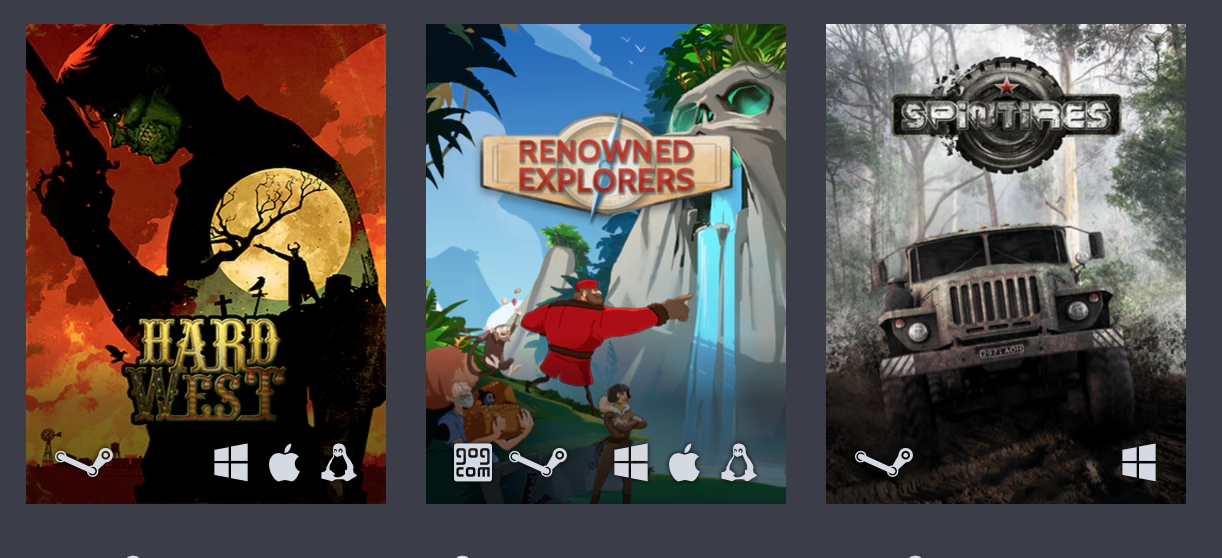
\includegraphics[scale=0.45]{bundlegames.png}
    \end{center}
    \footnotetext[1]{https://www.humblebundle.com}  
\end{frame}

\note[itemize]{
      \item Traditional approaches use ratings on individual items in
        recommender systems.
}


\iffalse
\begin{frame}{Publications}
  \Fontvi
  \begin{itemize}
    \item Related to thesis
      \begin{itemize}
        \Fontvi
        \item Mohit Sharma, Max Harper, and George Karypis. Learning from sets of items in
          Recommender Systems. International World Wide Web Conferences (WWW), 2017 (Under Review).
        \item Mohit Sharma and George Karypis. Matrix completion and item
          recommendations. Pacific-Asia Conference on Knowledge Discovery and
          Data Mining (PAKDD), 2017 (Under Review).
        \item Mohit Sharma, Jiayu Zhou, Junling Hu, and George Karypis.
          Feature-based factorized Bilinear Similarity Model for Cold-Start \TOPN
          Item Recommendation. SIAM International Conference on Data Mining (SDM), 2015. 
      \end{itemize}
    \item Other
      \begin{itemize}
        \Fontvi
        \item David C. Anastasiu, Evangelia Christakopoulou, Shaden Smith, Mohit
          Sharma, and George Karypis. Big Data and Recommender Systems. Big Data
          Novatica Special Issue, 2016.
        \item Vishwanathan N., Bandyopadhyay A., Fu H., Sharma M., Johnson K.,
          Mudge J. Ramaraj T., Onsongo G., Silverstein K., Jacob N., Le H.,
          Karypis G, and Hu W. Augmenting Chinese hamster genome assembly by
          identifying regions of high confidence.  Biotechnology Journal, 
          2016.
      \end{itemize}
  \end{itemize}
\end{frame}
\fi

\input{lfs_talk.tex}
%\input{lfs_proposal.tex}
%\input{matrixcompletion_slides.tex}
%\input{matrixcompletion_proposal.tex}
%\input{bilinear_slide.tex}

\begin{frame}
  \begin{center}
    \Huge{Questions?}
  \end{center}
  \note{1}
\end{frame}

\end{document}


